
%(BEGIN_QUESTION)
% Copyright 2010, Tony R. Kuphaldt, released under the Creative Commons Attribution License (v 1.0)
% This means you may do almost anything with this work of mine, so long as you give me proper credit

Anta at et venturiror er installert pa en damplinje for a male stromningen av hoytrykksdamp som kommer fra en kraftverkskjele og gar til en dampturbin (for a generere elektrisitet).  Entreprenorene som installerte mengdemaleren etterlot deg dette rotet:

$$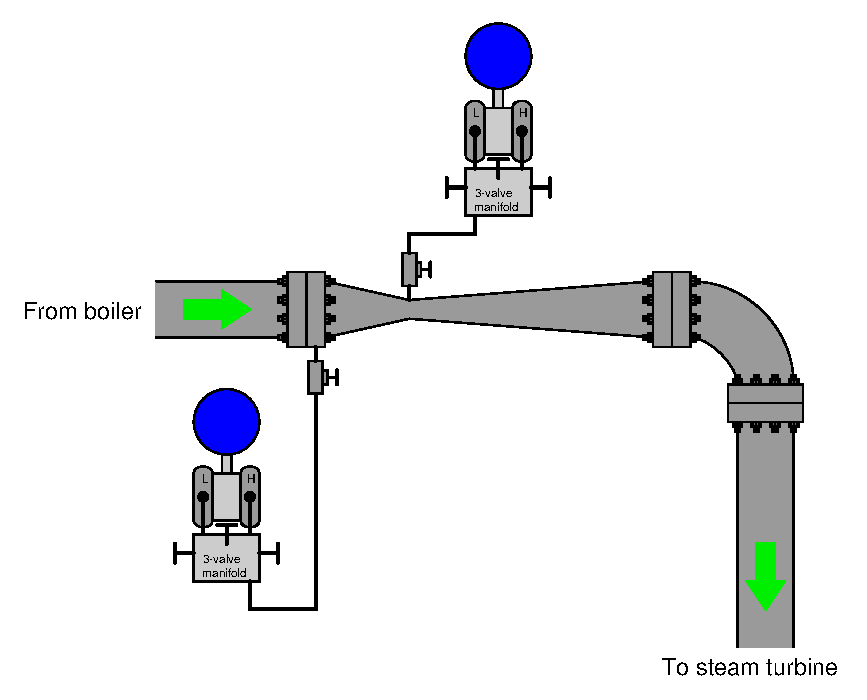
\includegraphics[width=15.5cm]{i00054x01.eps}$$

Forklar hva som er galt med denne installasjonen, og hva som ma gjores for a rette den.

\vfil

\underbar{file i00054}
\eject
%(END_QUESTION)





%(BEGIN_ANSWER)

Dette er et vurdert sporsmal -- ingen svar eller hint gis!

%(END_ANSWER)





%(BEGIN_NOTES)

Forst bor det bare vare en transmitter, ikke to.  A ha to transmittere er unodig komplisert, siden to signaler ma fores til kontrollsystemet, disse signalene trekkes fra hverandre for a komme frem til et differansetrykk, og deretter ma kvadratrotskarakteristikken gjores pa det beregnede $\Delta$P-signalet.  En transmitter er tilstrekkelig, med hoy- og lavtrykksuttak tilkoblet.

\vskip 10pt

Tradisjonelt har DP-transmittere vart montert {\it under} dampror, slik at kondensert vann kontinuerlig fyller begge impulslinjene og dermed ikke skaper noe hydrostatisk differansetrykk.  Det bor imidlertid bemerkes at montering over roret for damptjeneste er tillatt, sa lenge impulslinjene er korte i lengde (``close-coupled'') og store i diameter for a unnga muligheten for a fange en ``slug'' av kondensat langs sin lengde, som ville skjeve differansetrykkmalingen.

Som en praktisk sak kan det vare umulig a ``close-couple'' en DP-transmitter til et venturiror, hvis venturien er betydelig lang.  Close-coupling er generelt praktisk bare pa orifice-plate-installasjoner utstyrt med flensuttak, pa grunn av den relativt korte avstanden mellom trykkportene pa en typisk DP-transmitter.  Siden dette er tilfellet, er det langt mer sannsynlig at vi ma plassere DP-transmitteren under venturien i denne applikasjonen.

\vskip 10pt

Hvis DP-transmitteren er plassert under damproret, bor det ogsa monteres pafyllingstapper slik at impulslinjene kan forhandsfylles med vann nar de tas i bruk.  Dette eliminerer behovet for lang ventetid for mengdemalerens indikasjoner blir brukbare (vente pa at dampen kondenserer og fyller impulslinjene med vann).

\vskip 10pt

Her er en korrigert illustrasjon:

$$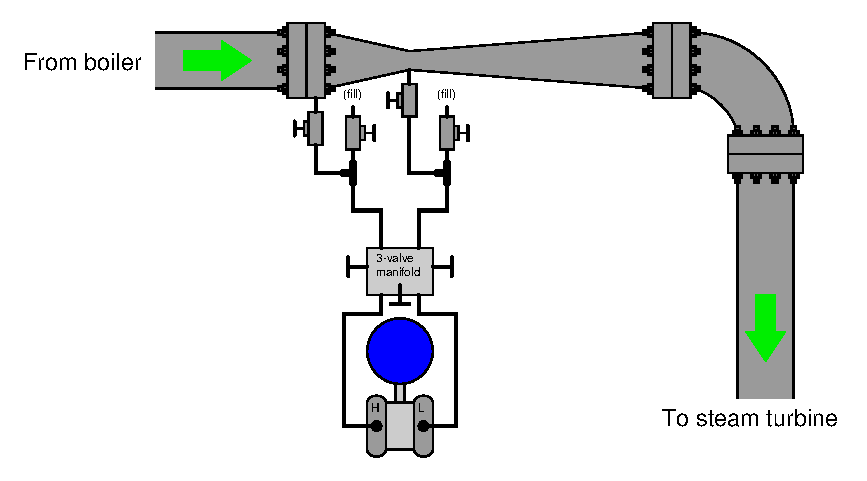
\includegraphics[width=15.5cm]{i00054x02.eps}$$

%INDEX% Measurement, flow: venturi tube

%(END_NOTES)


